\chapter{Background}
\label{sec:background}

\section{Reinforcement learning}

This entire section is descriptions of key concepts from a book on
Reinforcement Learning by Sutton and Barto \cite{sutton1998reinforcement}. If
no other reference is explicitly mentioned, statements are taken from this
book.

\subsection{The three tiers of machine learning}

In reinforcement learning (RL) an agent interacts with an environment and tries
to maximize how much \textit{reward} it can receive from the environment. To
maximize the reward in the long run might require short-time losses, making the
problem more complex than just maximizing for one step at a time. To find a
good strategy, commonly referred to as a \textit{policy}, the agent uses its
experience to make better decisions, this is referred to as
\textit{exploitation}. But, it must also find a balance between exploitation
and to also try out new things, i.e. \textit{exploration}. These features are
specific for RL and therefore distinguishes it from supervised and unsupervised
learning making it the third tier of machine learning.

\subsection{Main elements of RL}

Let $S_t$ be the state at time $t$, $R_t$ be the reward at time $t$, and $A_t$
the action at time $t$. The interaction between an agent and its environment in
RL is depicted in figure \ref{fig:rl_flowchart}. At time step $t$, the agent
reads the environment state and takes an action. The environment changes, maybe
stochastically, by responding with a new state $S_{t+1}$ and a reward $R_{t+1}$
at time $t+1$. 

\begin{figure}[h]
    \centering
    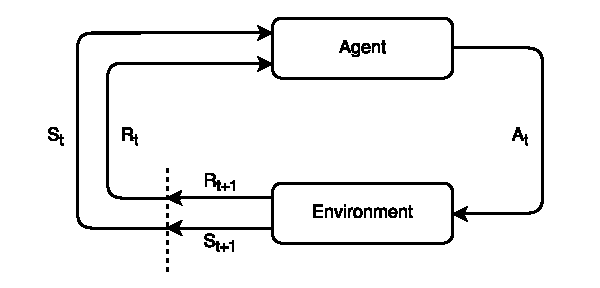
\includegraphics[]{res/agent_environment_interaction.pdf}

    \caption{Agent and environment interaction in RL. $S_t$, $R_t$, and $A_t$
             is the state, reward, and action at time $t$ \cite{sutton1998reinforcement}.}

    \label{fig:rl_flowchart}
\end{figure}

The quantity to maximize is often not the immediate rewards, but rather the
long term accumulated rewards. Let us call this quantity $G_t$, or
\textit{return}, for an agent at time $t$ up to some time $K$:

\begin{equation}
    G_t = \sum_{k=0}^K \gamma^k R_{t+k+1}
\end{equation}

Some problems imply that $K$ can go to infinity, and for $\gamma = 1$, $G_t$
can theoretically take infinite values. It is obviously problematic to maximize
something infinite and that is the reason for the $\gamma \in \left[0,
1\right]$ factor above that alleviates this problem if $\gamma < 1$ (proof
omitted). For lower values of $\gamma$ the agent tries to maximize short term
rewards, and for larger values long-term rewards. 

A policy is a function from the state of the environment to probabilities over
actions, i.e. the function that chooses what to do in any situation. Since a
reward is only short-term, a \textit{value function} tries to estimate the
total amount of reward that will be given in the long run for being in some
state and following some policy. To enable planning of actions in the
environment, RL algorithms sometimes use a \textit{model} in order to
explicitly build up an understanding of the environment. This is usually
referred to as \textit{model-based} RL in contrast to \textit{model-free}.

\subsection{Finite Markov Decision Processes}

In a RL scenario where the environment has a finite number of states, there is
a finite number of actions, and the Markov property holds is called a
\textit{finite Markov Decision Process} (finite MDP). The dynamics of a finite
MDP are completely specified by the probability distribution:

\begin{equation}
    p(s', r|s, a) = P(S_{t+1} = s', R_{t+1} = r | S_t = s, A_t = a)
\end{equation}

Important functions and terminology that is used throughout RL includes the
\textit{state-value function} (abbreviated as value function) and the
\textit{action-value function}. The state-value function with respect to some
policy informally gives how good a state is to be in given that
the policy is followed thereafter:

\begin{equation}
    v_\pi(s) = \mathbb{E}_\pi\left[G_t|S_t=s\right] = \mathbb{E}_\pi\left[\sum_{k=0}^\infty \gamma^k R_{t+k+1}|S_t=s\right]
\end{equation}

To compare the value of different actions in some state, given that you thereafter follow some policy $\pi$,
is given by the action-value function:

\begin{equation}
    q_\pi(s, a) = \mathbb{E}_\pi\left[G_t|S_t=s,A_t=a\right] = \mathbb{E}_\pi\left[\sum_{k=0}^\infty \gamma^k R_{t+k+1}|S_t=s,A_t=a\right]
\end{equation}

According to RL theory there is always an optimal policy
\cite{sniedovich1986new}, i. e. that gives the highest possible expected return
given any state. This is often denoted with $*$ and has the corresponding value
and action-value functions $v_*(s)$ and $q_*(s, a)$. Given the optimal value or
action-value function, it is (depending on the problem) easy to infer the
optimal policy, therefore a common approach is to first approximate either of
these functions.

\subsection{Policy and value iteration}

One exact method to find the optimal policy, at least in the limit, is called
\textit{policy iteration}. This builds on two alternating steps, the first
called \textit{iterative policy evaluation}. This estimates a value function
given some policy and starts from a random value function $v_0$, except for any
terminal state $s_K$ for which are assigned $v_0(s_K) = 0$. By $v_k$ is meant
the value function estimate at iteration $k$. Then we iteratively update new
value functions for each step:

\begin{align*}
    v_{k+1}(s) &= \mathbb{E}\left[R_{t+1} + \gamma v_{k}(S_{t+1}) | S_t=s \right] \\
               &= \sum_a \pi (a|s) \sum p(s', r|s, a) \left[r + \gamma v_k(s')\right]
\end{align*}

As can be seen, the dynamics $p(s', r|s, a)$ needs to be known, which of course
is not always the case. The next step is called \textit{policy improvement} and for this
we first need to calculate the action-state function given the current policy
$\pi$:

\begin{align*}
    q_\pi(s, a) &= \mathbb{E}\left[R_{t+1} + \gamma v_\pi(S_{t+1}) | S_t=s, A_t = a \right] \\
                &= \sum_{s', r} p(s', r|s, a) \left[r + \gamma v_\pi(s')\right]
\end{align*}

Given this, an improved policy $\pi'$ is attained by:

\begin{equation}
    \pi'(s) = \text{arg}\max_a q_\pi(s, a)
\end{equation}

Iteratively performing these two steps will eventually converge to the optimal
policy \cite{puterman1979convergence}. There is an alternative way that is done by only approximating the
value function, called \textit{value iteration}:

\begin{align*}
    v_{k+1}(s) &= \max_a \mathbb{E}\left[R_{t+1} + \gamma v_k(S_{t+1}) | S_t=s, A_t = a \right] \\
             &= \max_a \sum_{s', r} p(s', r|s, a) \left[r + \gamma v_k(s')\right]
\end{align*}

After convergence to some value function $v$, the optimal policy is found by:

\begin{equation}
    \pi'(s) = \text{arg}\max_a \sum_{s', r} p(s', r|s, a) \left[r + \gamma v(s')\right]
\end{equation}

\subsection{Monte Carlo methods and Temporal-Difference learning}

Policy and value iteration are exploring the entire state-action space and
finds an optimal policy if the dynamics of the environment are known. Sometimes
we are dealing with samples from interacting with a system, and where we do not
know the dynamics. For these cases, we can instead estimate the action-value
function given a policy. This can be done by \textit{Monte Carlo methods} which
in its simplest form is averaging of returns for samples that we have attained.
The other method is \textit{Temporal-difference methods} which estimates an error
for each observed reward and updates the action-value function with this. To be
more precise, one famous example of a time difference method is
\textit{Q-learning} and the updates are done according to:

\begin{equation}
    Q(S_t, A_t) \leftarrow Q(S_t, A_t) + \alpha \left[ R_{t+1} + \gamma \max_a Q(S_{t+1}, a) - Q(S_t, A_t) \right]
\end{equation}

Q-learning is an example of an \textit{off-policy} method. This means that you
can use a second, or derived, policy for exploration, but the algorithm still
finds the optimal policy. The other family of methods is called
\textit{on-policy} methods and are characterized by that the expectation being
maximized is with respect to the exploring policy. In contrast to this the
expectation in the off-policy case is only dependent on the environment.

\section{Neural networks}

\subsection{Basic idea}

The simplest neural network could be considered to be a linear transformation
of some data points $X$:

\begin{equation}
    X_1 = WX + B
\end{equation}

Since for some column in $X$, all its values influence all the values in the
same column in $X_1$, the \textit{input layer} $X$ and \textit{layer} $X_1$ are
said to be \textit{fully connected}. The convention of describing neural
networks with layers comes from the inspiration of physical neurons arranged in
layers although the description is not as apparent when describing the networks
in this fashion. The above transformation is obviously restricted to learning
linear transformations, so to learn non-linear functions, a
non-linear \textit{activation-function} is added:

\begin{equation}
    X_1 = f(WX + B)
\end{equation}

To learn more complex functions, transformations can be recursively stacked:

\begin{align}
    X_2 &= f(W_1X_1 + B_1)\\
    ...\\
    Y_{k+1} &= f(W_kX_k + B_k)
\end{align}

A loss function is a function $\ell : f, \mathbb{R}^d \longmapsto \mathbb{R}$,
where $f$ is the neural network and $\mathbb{R}^d$ is some data. Usually, the
data are inputs to the network, often along with corresponding target values.
This specifies the error, and implicitly the wanted behavior of the network. By
all parts being differentiable we can specify the loss function and calculate
its derivatives with respect to all the parameters $W, W_1,...$ and $B, B_1,
...$.  Using this we can then minimize the loss using gradient descent. A
common and effective way to do this is called \textit{back-propagation}
\cite{williams1986learning}.  The first layer $X$ is commonly referred to as
the input layer and the last layer as the output layer. The intermediate values are
referred to as hidden layers.

\subsection{Common activation functions}

Two common activation functions include \textit{tanh} and \textit{Rectified
Linear Unit} (ReLU) \cite{jarrett2009best} shown in figure \ref{fig:tanh_relu}. The tanh function is defined as:

\begin{equation}
    \tanh(x) = \frac{2}{1+e^{-x}} - 1
\end{equation}

The ReLU is defined as:

\begin{equation}
    \text{relu}(x) = \max (0, x)
\end{equation}

Another addition to the family of activation functions is the
\textit{exponential linear unit} (ELU) \cite{clevert2015fast} which has the
benefit of propagating the gradient also for negative input values since the
limit for large negative input values is $-1$ rather than $0$ as for the ReLU.
This was shown to speed up training and lowering classification test errors.
The ELU is defined as (with $\alpha$ usually being set to $1.0$):

\begin{equation}
    f(\alpha, x) =
    \begin{cases}
        \alpha (e^{x} - 1) & \text{if } x < 0 \\
        x & \text{if } x \geq 0
    \end{cases}
\end{equation}

For classification networks, a common function to have in the output layer is
the softmax function shown in figure \ref{fig:softmax}. A property of the
softmax is that all values will be output in the range $[0, 1]$ and sum to one,
making it conveniently interpreted as probabilities of different classes or
categories. The mathematical definition is for a set $x_1, ..., x_K$:

\begin{equation}
    \text{softmax}(x_k|x_1, ..., x_K) = \frac{e^{x_k}}{\sum_{i=1}^K e^{x_i}}
\end{equation}

\begin{figure}[h]
    \centering
    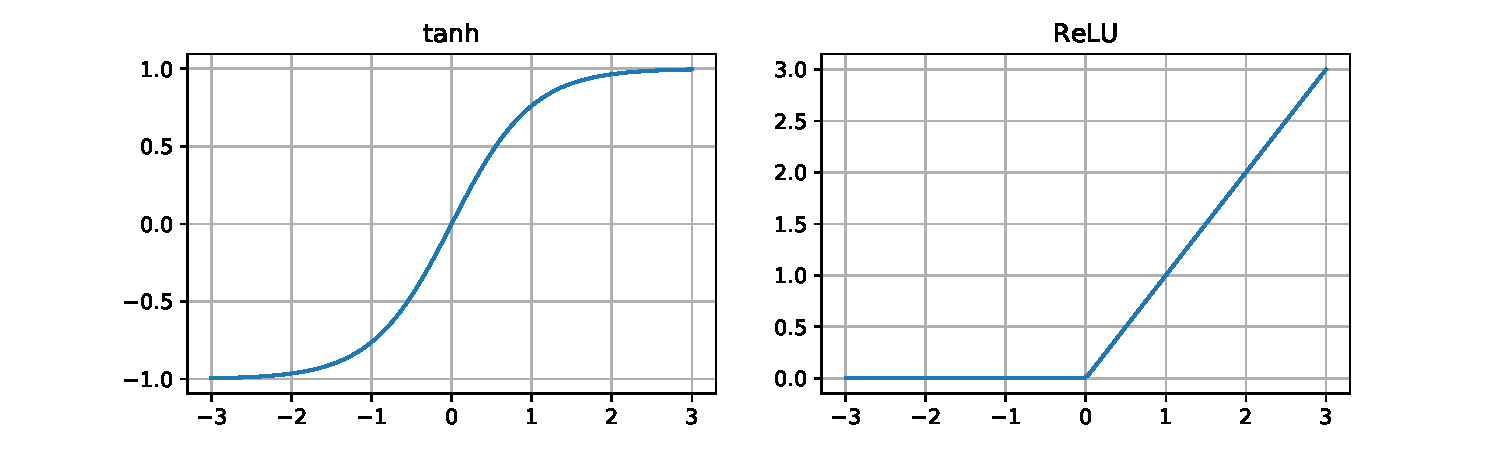
\includegraphics[width=0.8\textwidth]{res/relu_tanh.pdf}

    \caption{Common activation functions for neural networks.}

    \label{fig:tanh_relu}
\end{figure}

\begin{figure}[h]
    \centering
    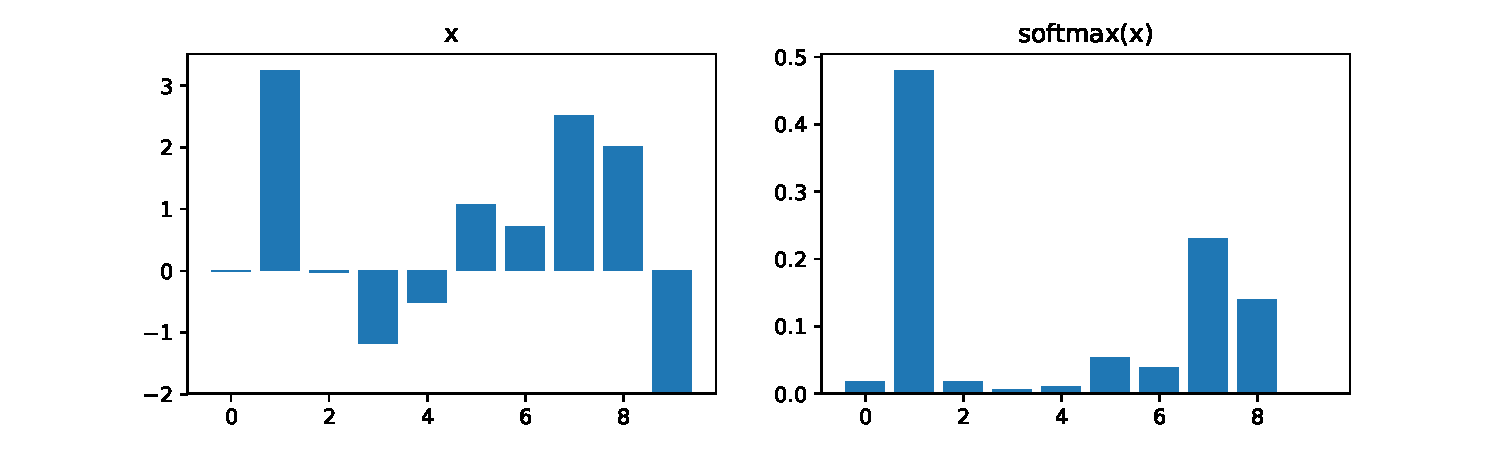
\includegraphics[width=0.8\textwidth]{res/softmax.pdf}

    \caption{Softmax function commonly used to convert a set of numbers $\in
    \mathbb{R}$ to probabilities of a discrete set of categories.}

    \label{fig:softmax}
\end{figure}

\subsection{Weight sharing}

In order to construct effective models with less number of parameters the fact
is used that some features are invariant of where in the data they are, e.g.
the pattern $1, 2, 3, 4$ in the beginning, middle, or the end of the data. To
this end, convolutions are used (where $*$ is the convolution operator):

\begin{equation}
    y = w * x + b
\end{equation}

These kind of networks are usually referred to as \textit{convolutional neural
networks} (CNN) \cite{lecun1989backpropagation}. The notation becomes a bit
more tricky here since the convolutions are commonly done in two dimensions
with 3-dimensional kernels ($w$). These are commonly used in neural networks
for images. It is common to use an other form of layer in conjunction with
convolutional layers called \textit{pooling} layers. These are used to reduce
the dimensionality from one layer to another and are very similar to
convolutions, but instead of kernels with varying weights, a max operation
\cite{huang2007unsupervised} or average operation \cite{lecun1998gradient} is
applied (average pooling is a kernel with all weights being equal).

\subsection{Optimizers}

A method commonly used for optimizing neural networks is called Adam
\cite{kingma2014adam}. Updates to parameters of the function with loss function
$f(\theta)$ are done by first and second order estimates of the gradients $g_t
= \nabla_{\theta_t} f(\theta_{t-1})$. The current timestep is annotated $t$ and
starts with $t = 1$, this is used to bias-correct the first and second order
estimates:

\begin{equation}
    m_t = \beta_1 m_{t-1} + (1 - \beta_1) g_t
\end{equation}

\begin{equation}
    v_t = \beta_2 v_{t-1} + (1 - \beta_2) g_t^2
\end{equation}

\begin{equation}
    \mathbb{E}\left[g \right] \approx \hat{m}_t = \frac{m_t}{1- \beta_1^t}
\end{equation}

\begin{equation}
    \mathbb{E}\left[g^2 \right] \approx \hat{v}_t = \frac{v_t}{1- \beta_2^t}
\end{equation}

Here $\beta_1, \beta_2 \in [0, 1)$ are hyperparameters. The updates are done
with stepsize $\alpha$ according to ($\epsilon >0$ to ensure no division by zero):

\begin{equation}
    \theta_t = \theta_{t-1} - \alpha \frac{\hat{m}_t}{\sqrt{\hat{v}_t - \epsilon}}
\end{equation}

Adam can be seen as a generalization of RMSProp where $\beta_1 = 0$
\cite{tieleman2012lecture} which implies that only a running second order
estimate is used. This has been successfully used for training of on-policy
algorithms \cite{mnih2016asynchronous} where gradients from previous policies
included in the running mean might not be suitable for current policy updates.
Earlier commonly used methods include Adadelta \cite{zeiler2012adadelta},
Adagrad \cite{duchi2011adaptive}, and momentum \cite{qian1999momentum}.


\subsection{Avoiding overfitted networks}

A classical approach to regularize neural networks is adding a scaled L2-norm
of the parameters to the loss. Another way shown to be effective, both for
fully connected and convolutional neural networks, is called dropout
\cite{srivastava2014dropout}. During training time, units are with probability
$p$ set to zero and non-zeroed outputs are scaled by $1/p$. Effectively, this
means inference during training time is done using random subgraphs of the
neural network, and inference during test time is done by average voting from a
collection of those subgraphs. To alleviate the problem of overfitting when
using images, it is common to use data augmentation, i. e. applying random
scaling, translations, noise etc. to the images (e.g.
\cite{ciregan2012multi,simard2003best,krizhevsky2012imagenet}). Another
approach is to synthetically generate a larger image database by overlaying
parts of the images with patches of other objects \cite{ghadirzadeh2017deep}.

\subsection{Batch normalization}

As the weights in one layer changes during training, the following layers have
to adapt to this change. In fact, later layers constantly have to adopt to
changes in any of the previous layers during training, something called
\textit{internal covariance shift}. It was shown that this problem can be
solved by adding intermediate normalization layers, called \textit{batch
normalization} \cite{ioffe2015batch}. These layers whiten the activations of
the previous layer, i. e. element-wise subtraction of the mini-batch mean and
divide by the square root of the variance. Since the statistics are calculated
per mini-batch, they argue that this acts as a regularizer, and they
empirically show that dropout in some cases are no longer needed. They argue
that this is due to that the representation of one sample will shift
differently depending of the other samples in the mini-batch. For some cases,
whitening the outputs of the previous layer decreases what the next layer can
represent, e. g. not saturating the sigmoid function in the subsequent layer.
To alleviate this problem, the authors propose learnable parameters that ensure
that the normalization layer, if needed, can represent the identity function.
During inference, normalization is done on population estimates of the mean and
variance. These population estimates are inferred using running mean and
variance estimates attained during training. Using batch normalization showed
to decrease the number of training steps by a factor of 14 for some cases, and
improving the test errors of previous state-of-the-art networks.

\section{Reinforcement Learning for Robotics}

\subsection{Q-function estimation using neural networks}

For continuous state spaces, Q-learning can no longer be solved by tabular
methods, and in practice many discrete state space problems are also too large
to be represented and learned this way. Therefore it was proposed that the
Q-function be estimated using a neural network updated in a standard Q-learning
fashion, i. e. for one sample at a time after one interaction with the
environment \cite{riedmiller1999concepts}. Here, the action maximizing the
value going from the successor state is found by searching since there is a
finite amount of actions. However this was shown to need several tens of
thousands of episodes before convergence to optimal or near optimal policies
\cite{riedmiller1999concepts}. Instead of updating the Q-function on-line one
sample at a time, all state-action-successor state tuples $(s, a, s')$ can be
stored and used to update the network off-line using batches, which was found
to converge faster \cite{riedmiller2005neural}.

\subsection{Recent progress in the discrete action setting}

For playing the board game Go, a four-step process was proposed
\cite{silver2016mastering}. The first step was to train a policy in a
supervised fashion predicting expert moves. Thereafter, the policy was improved
by playing games against previous iterations of the same policy and updating
using policy gradient methods. A value function was then estimated given the
best policy from the previous step, this was then used to perform Monte Carlo
tree search to find the best action. The resulting policy/algorithm later beat the world
champion Lee Sedol \cite{deepmind_2017}.

For continuous state spaces in contrast to Go, namely images from the screen of
video games, a deep-Q-network (DQN) was proposed \cite{mnih2013playing}. Here,
a sequence of images (neighboring in time) from the games were input to a
convolutional neural network. The final layer was a fully connected layer which
outputs a state-action estimate for each action. This enabled faster selection
of the optimal action due to one single forward pass of the network. The
network was trained and evaluated on seven Atari games, surpassing a human
expert in three of the games, and surpassing previous methods in six of the
games.


\subsection{Normalized Advantage Functions (NAF)}

In order to extend Q-learning to continuous state and action spaces, Gu et al.
\cite{gu2016continuous} proposes a relatively simple solution called normalized
advantage functions (NAF). They argue after doing simulation experiments that
this algorithm is an effective alternative to recently proposed actor-critic
methods and that it learns faster with more accurate resulting policies. First,
the action-value function is divided into a sum of the value function $V$ and
what they call an advantage function $A : \mathbb{R}^d \longmapsto \mathbb{R}$:

\begin{equation}
    Q(\mathbf{x}, \mathbf{u}) = A(\mathbf{x}, \mathbf{u}) + V(\mathbf{x})
\end{equation}

Here, $\mathbf{x}$ is the state of the environment and $\mathbf{u}$ are
controls or actions. The advantage function is a quadratic function of $u$:

\begin{equation}
    A(\mathbf{x}, \mathbf{u}) = -\frac{1}{2}(\mathbf{u} - \mathbf{\mu(x)})^T\mathbf{P(x)}(\mathbf{u} - \mathbf{\mu(x)})
    \label{eq:advantage_function}
\end{equation}

There are more terms that need to be defined, but first consider equation
(\ref{eq:advantage_function}). The matrix $\mathbf{P}$ is a positive-definite
matrix, this makes the advantage function have its maximum when $\mathbf{u =
\mu(x)}$.  The purpose of $\mu$ is to be a greedy policy function, thus
$\mathbf{Q}$ is maximized when $\mathbf{u}$ is the greedy action. The purpose
of this is that given an optimal $Q$, we do not need to search for the optimal
action, since we know $\mathbf{\mu}$. Now the definition of $\mathbf{P}$:

\begin{equation}
    P(\mathbf{x}) = \mathbf{L(x)L(x)}^T
\end{equation}

Here, $\mathbf{L}$ is a lower-triangular matrix where diagonal entries are
strictly positive.

After these definitions, we are left with estimating the functions $V$,
$\mathbf{\mu}$, and $\mathbf{L}$. To this end the authors use a neural network,
here shown in figure \ref{fig:naf-net}. The $\mathbf{L}$ output is fully
connected with the previous layer and not passed through an activation function
(it is linear). The diagonal entries of L are exponentiated. Hidden layers
consisted of 200 fully connected units with rectified linear units (ReLU) as
activation functions except for $\mathbf{L}$ and $A$ as already defined.

\begin{figure}[h]
    \centering
    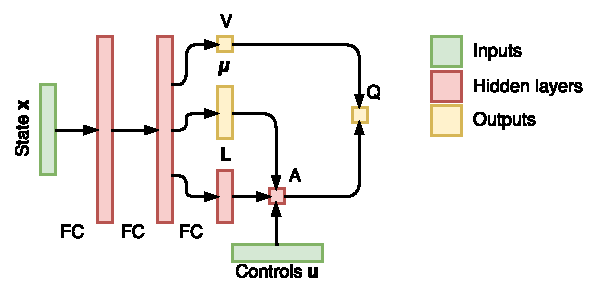
\includegraphics[width=1.0\textwidth]{res/naf-net.pdf}

    \caption{Neural network design for NAF \cite{gu2016continuous}. The
    activation function to $V$ was not specified. The tanh activation was added
    in figure due to Gu et al. \cite{gu2016deep} using it in order to have
    bounded actions for safety reasons.}

    \label{fig:naf-net}
\end{figure}

The NAF algorithm is listed in algorithm \ref{algo:naf}. All collected experiences
are stored in a replay buffer that optimization is run against. Exploration is done
by adding noise to the current greedy policy $\mathbf{\mu}$.

\begin{algorithm}[!h]
    \caption{NAF algorithm}
    \begin{algorithmic}
        \STATE{Randomly initialize network $Q(x, u|\theta)$}
        \STATE{Initialize target network $Q'$, $\theta' \leftarrow \theta$}
        \STATE{Initialize replay buffer $R \leftarrow \emptyset$}
        \FOR{episode $= 1$ to $M$}
            \STATE{Initialize random process $\mathcal{N}$ for action exploration}
            \STATE{Receive initial exploration state $x_1$}
            \FOR{$t = 1$ to $T$}
                \STATE{Select action $\mathbf{u_t = \mu(x_t|\theta) + \mathcal{N}_t}$}
                \STATE{Execute $\mathbf{u_t}$ and observe $r_t$ and $\mathbf{x}_{t+1}$}
                \STATE{Store transition $(\mathbf{x}_t, \mathbf{u}_t, r_t, \mathbf{x}_{t+1})$ in $R$}
                \FOR{iteration $= 1$ to $I$}
                    \STATE{Sample a random minibatch of $m$ transitions from $R$}
                    \STATE{Set $y_i = r_i + \gamma V'(\mathbf{x}_{i+1}|\theta')$}
                    \STATE{Update $\theta$ by minimizing the loss:
                           $L = \frac{1}{N}\sum_i (y_i - Q(\mathbf{x}_i, \mathbf{u}_i|\theta))^2$}
                    \STATE{Update target network $\theta' \leftarrow \tau \theta + (1 - \tau)\theta'$}
                \ENDFOR
            \ENDFOR
        \ENDFOR
    \end{algorithmic}
    \label{algo:naf}
\end{algorithm}

\subsection{Distributed real-world learning using NAF}
\label{sec:distributed_naf}

Real-world experiments were done by Gu et al. \cite{gu2016deep} on door opening
tasks using the NAF algorithm and 7-DoF torque controlled arms. They extended
the algorithm to be distributed on several robots/collectors and one separate
trainer thread on a separate machine. They state that this was the first
successful real-world experiment with a relatively high complexity problem
without human demonstration or simulated pretraining. They used the layout of
the network shown in figure \ref{fig:naf-net} but with hidden layers of 100
units each. Also, in this article it was explicitly mentioned that the
activation functions for the policy $\mathbf{\mu}$ was tanh in order to bound
the actions. The state input consisted of the arm pose and target pose. The
target pose was known from attached equipment. The modified version of NAF is
listed in algorithm \ref{algo:async_naf}.

The authors conclude that there was an upper bound on the effects of
parallelization, but hypothesize that the speed of the trainer thread has a
limiting factor in this matter. They used CPU for training the neural network
so instead using a GPU might increase the effect of more collectors.

\begin{algorithm}[!h]
    \caption{Asynchronous NAF - $N$ collector threads and $1$ trainer thread}
    \begin{algorithmic}
        \STATE{// trainer thread}
        \STATE{Randomly initialize network $Q(\mathbf{x}, \mathbf{u}|\theta)$}
        \STATE{Initialize target network $Q'$, $\theta' \leftarrow \theta$}
        \STATE{Initialize shared replay buffer $R \leftarrow \emptyset$}
        \FOR{iteration $= 1$ to $I$}
            \STATE{Sample a random minibatch of m transitions from $R$}
            \STATE{Set $y_i = \begin{cases}r_i+\gamma V'(x_i|\theta) &\text{ if } t_i < T,\\r_i &\text{ if } t_i = T\end{cases}$}
            \STATE{Update $\theta$ by minimizing the loss:
                   $L = \frac{1}{m} \sum_i (y_i - Q(\mathbf{x}_i, \mathbf{u}_i|\theta))^2$}
            \STATE{Update the target network: $\theta' \leftarrow \tau\theta + (1-\tau)\theta'$}
        \ENDFOR
        \STATE{// collector thread $n$, $n = 1...N$}
        \FOR{episode $= 1$ to $M$}
            \STATE{Sync policy network weights $\theta_n \leftarrow \theta$}
            \STATE{Initialize a random process $\mathcal{N}$ for action exploration}
            \STATE{Receive initial observation state $x_1$}
            \FOR{$t = 1$ to $T$}
                \STATE{Select action $\mathbf{u}_t = \mathbf{mu}$}
                \STATE{Execute $\mathbf{u}_t$ and observe $r_t$ and $\mathbf{x}_{t+1}$}
                \STATE{Send transition $(\mathbf{x}_t, \mathbf{u}_t, r_t, \mathbf{x}_{t+1}, t)$ to $R$}
            \ENDFOR
        \ENDFOR
    \end{algorithmic}
    \label{algo:async_naf}
\end{algorithm}

\subsection{Deep deterministic policy gradient}
\label{sec:ddpg}

An alternative continuous Q-learning method to the NAF formulation is an
actor-critic approach called Deep Deterministic Policy Gradient (DDPG)
\cite{lillicrap2015continuous}. Separate networks are defined for the
Q-function (critic) and a deterministic policy $\mu$ (actor), and the
target quantity for the critic to predict becomes:

\begin{equation}
    Q^\mu(s_t, u_t) = \mathbb{E}_{s_{t+1}}\left[ r_t + \gamma Q^\mu(s_{t+1}, \mu (s_{t+1})) \right]
\end{equation}

The Q-function is trained by optimizing the temporal difference error, and the
policy is trained by updating its parameters $\theta_\mu$ according the policy
gradient. The policy gradient in equation (\ref{eq:ddpg_policy_gradient}) was
shown to be the gradient of the expected value of the return with respect to
its parameters \cite{lever2014deterministic}. The expected return is below
notated $J$.

\begin{align}
    \nabla_{\theta_\mu}J &= \nabla_{\theta_\mu} \mathbb{E}_s \left[\sum_{t=1}^\infty \gamma^{t - 1} r_t \right] \\
                         &= \mathbb{E}_s \left[\nabla_u Q(s, \mu(s)) \nabla_{\theta_\mu} \mu(s|\theta_\mu) \right] \label{eq:ddpg_policy_gradient}
\end{align}

Note that the product in the expectation in equation
\ref{eq:ddpg_policy_gradient} is a matrix multiplication. The left hand side is
a $1 \times n_u$ matrix where $n_u$ is the dimensionality of the actions. The
right hand side is a $n_u \times n_\theta$ matrix, where $n_\theta$ is the
number of parameters in the actor model. The expectation is over the states $s$
in the environment, and can be approximated by drawing $N$ samples from
interactions with the environment:

\begin{equation}\label{eq:policy_gradient}
    \nabla_{\theta_\mu}J = \frac{1}{N} \sum_{n=1}^N \nabla_a Q(s, \mu(s)) \nabla_{\theta_\mu} \mu(s|\theta_\mu)
\end{equation}

Since the Q-network fits to its own values in a recursive way, it was
experienced to be unstable. This was solved by having separate target networks
$Q'$ and $\mu'$. Mean square error loss $\mathit{L}$ of the temporal
differences errors were calculated by:

\begin{equation}
    y_i = r_i + \gamma Q'(s_{i+1}, \mu'(s_{i+1}))
\end{equation}

\begin{equation}
    \mathit{L} = \frac{1}{N} \sum_{i=1}^N \left[y_i - Q(s_i, u_i)) \right]^2
\end{equation}

Target networks were then slowly updated by $\tau < 1$:

\begin{equation}
    \theta_{\mu'} = \tau \theta_{\mu} + (1 - \tau) \theta_{\mu'}
\end{equation}
\begin{equation}
    \theta_{Q'} = \tau \theta_{Q} + (1 - \tau) \theta_{Q'}
\end{equation}

The networks were setup to have two hidden layers of $400$ and $300$ units
each.  All hidden layers had ReLU activation functions, output of the action
network was bounded by using tanh activation functions. The method was shown to
solve a variety of task with continuous controls. Instead of performing the
matrix multiplication in equation (\ref{eq:policy_gradient}) explicitly when
using computational graph libraries, actor parameters $\theta_\mu$ are easily updated by
maximizing the quantity (keeping critic parameters $\theta_Q$ fixed):

\begin{equation}
    Q(s, \mu(s|\theta_\mu)|\theta_Q)
\end{equation}

\subsection{Guided Policy Search}

Guided policy search (GPS) \cite{levine2013guided} maximizes the expected
return $J(\theta)$ using trajectories $\zeta^i_{1:T} = \{(x_1^i, u_1^i), ...,
(x_T^i, u_T^i)\}$ and the respective rewards $\{r_1^i, ..., r_T^i\}$. The
superscript $i$ denotes the sample. In order to use trajectories from previous
policies, importance sampling is used and the quantity to maximize is becomes:

\begin{equation}
    \mathbb{E}[J(\theta)] \approx \sum_{t=1}^T \frac{1}{Z(\theta)} \sum_{i=i}^m \frac{\pi_\theta(\zeta^i_{1:t})}{q(\zeta^i_{1:t})}r_t^i
\end{equation}

Here $q(\zeta^i)$ is the probability of the trajectory $\zeta^i$ under the
distribution it was sampled from. The distribution $\pi_\theta$ gives the
probability of a sequence of the current policy parameterized by $\theta$. The
GPS algorithm iteratively maximizes this expectation and provides new guiding
samples by optimizing sampled trajectories using methods such as
\textit{iterative Linear Quadratic Regulator} (iLQR) \cite{tassa2012synthesis}
or \text{Policy Improvement with Path Integrals} ($\mathbf{PI}^2$)
\cite{theodorou2010generalized}. The found locally optimal trajectories can be
added as guiding samples in the above expectation.

\subsection{Asynchronous Advantage Actor-Critic (A3C)}

An on-policy actor-critic method was proposed that distributes the training
and exploration in simulated environments over several CPU cores
\cite{mnih2016asynchronous}. Each thread executes a sequence of actions and
then calculates the gradients, given that sequence, which are then sent to a
central parameter thread. The actor output $\pi(a|s)$ is parameterized as a Gaussian distribution
with a mean vector $\mathbf{\mu}$ and covariance matrix $\sigma\mathbf{I}$ where $\mathbf{\mu}$
and $\sigma$ are outputs from the actor network. Here $\pi(a|s)$ is the probability of the action $a$ given
some state $s$.
During exploration, actions $a_1, ..., a_T$ given states $s_1, ..., s_T$ are sampled from this distribution and the quantity being maximized
is:

\begin{equation}
    \ell(a_{1:T}, s_{1:T}, \theta_\pi, \theta_V) = \sum_{t=1}^T \log \pi (a_t|s_t, \theta_\pi) (R_t - V(s_t|\theta_V))
\end{equation}

Here $V$ is the critic network, and $R_t$ is the estimated return given by:

\begin{equation}
    R_t =
    \begin{cases}
        r_t + V(s_{t+1}|\theta_V) & \text{if } t = T\\
        r_t + R_{t+1} & \text{if } t < T
    \end{cases}
\end{equation}

In the central thread, gradients are applied to the parameters and local models
then update their parameters by querying the central thread. This was shown to
solve a range of manipulation tasks in simulation, although the authors are
somewhat vague about the results for the continuous action case. For the
discrete action case, the formulation differs somewhat, but results show a
substantial cut in training time on Atari games when using 16 CPU cores
compared to the original method where a GPU is used \cite{mnih2013playing}.

\subsection{Prioritized experience replay}
\label{sec:prio_sampling}

When randomly sampling experiences from a replay buffer, one alternative is to
sample from a uniform distribution. However, if samples are sampled from a
distribution where experiences with larger temporal-difference errors are more
likely to be chosen, training times can be reduced with resulting policies that
outperform those trained by uniform sampling \cite{schaul2015prioritized}. Let
$R_{t}$ be the reward at time $t$, $Q(S_t, A_t)$ the Q-function of state $S_t$
and action $A_t$ at time $t$ and $V(S_t)$ the value function for $S_t$ at time
$t$. Given a sample tuple $x_i = (S_t, S_{t+1}, A_t, R_{t+1})$, let the
temporal-difference error for this sample to be defined as:

\begin{equation}
    \delta_i = Q(S_{t}, A_t) - \left[ R_{t+1} + \gamma V(S_{t+1}) \right]
\end{equation}

Define a priority $p_i$ of sample $x_i$ as:

\begin{equation}
    p_i = |\delta_i| + \epsilon
\end{equation}

Here $\epsilon > 0$ ensures all priorities are strictly positive. Sample experiences
according to the probability:

\begin{equation}
    P(i) = \frac{p_i^\alpha}{\sum_k p_k^\alpha}
\end{equation}

The hyperparameter $\alpha \geq 0$ enforces more uniform probabilities for values close to
zero and more non-uniform probabilities for larger values.

Since the gradient is biased by a biased choice of samples, the magnitude of
the gradient with respect to each sample $x_i$ can be weighted by:

\begin{equation}
    w_i = \left( \frac{1}{P(i)} \right)^\beta
\end{equation}

The parameter $\beta \geq 0$ can be varied during training, and it is argued that
the unbiased gradients are more important towards the end when the policy is
converging. They varied this parameter reaching $\beta = 1$ only towards the
end of the training. It is not clear from the article but it is assumed that
training starts with $\beta = 0$.

\section{Spatial softmax in pose estimation}

Levine et al. \cite{levine2016end} proposed an architecture for a CNN that
gives pose estimates for robotic manipulation tasks. After the last
convolutional layer, a softmax is applied, but only normalized over each
kernel's response map, called \textit{spatial softmax}:

\begin{equation}
    s_{cij} = \frac{e^{a_{cij}}}{\sum_{i',j'} e^{a_{ci'j'}}}
\end{equation}

Here, $a_{cij}$ is the output of the $c$:th kernel at coordinate $ij$. After
this, they calculate the expected 2D position for each feature, which they
argue is better suited for pose estimation. The expected 2D position is
expressed as a tuple $(f_{cx}, f_{cy})$ calculated according to:

\begin{align}
    f_{cx} &= \sum_{i,j} s_{ij} x_{ij} \\
    f_{cy} &= \sum_{i,j} s_{ij} y_{ij}
\end{align}

The scalar value $x_{ij}$ is the position in image space of the pixel at coordinate
$(i, j)$. This can reasonably easy be simplified to a matrix multiplication with constant
weights from each of the response maps. Arguably, it could also be possible to rewrite the
above expressions as:

\begin{align}
    f_{cx} &= \sum_{i,j} i s_{ij} \\
    f_{cy} &= \sum_{i,j} j s_{ij}
\end{align}

As a measure of certainty of the expected position, is was proposed to use the
spatial softmax output at the expected position \cite{finn2016deep2}. Other
possible methods are naturally the estimated variance of the 2D position as
well as the maximum output of the spatial softmax.
